\documentclass[conference]{IEEEtran}
\IEEEoverridecommandlockouts

\usepackage{cite}
\usepackage{amsmath,amssymb,amsfonts}
\usepackage{graphicx}
\usepackage{textcomp}
\usepackage{xcolor}
\usepackage{booktabs}
\usepackage{url}
\usepackage[colorlinks=true,linkcolor=blue,citecolor=blue,urlcolor=blue]{hyperref}

\def\BibTeX{{\rm B\kern-.05em{\sc i\kern-.025em b}\kern-.08em
    T\kern-.1667em\lower.7ex\hbox{E}\kern-.125emX}}

\begin{document}

\title{Transfer Learning for Cross-Climate Building Energy Prediction: Investigating Data Efficiency and Generalization Across Climate Zones}

\author{
\IEEEauthorblockN{Shree Santosh Yadav}
\IEEEauthorblockA{\textit{School of Computer Science and Engineering} \\
\textit{RV University}\\
Bengaluru, India \\
USN: 1RUA24CSE0436 \\
shreesantoshyadavbtech24@rvu.edu.in}
\and
\IEEEauthorblockN{Samyak Jain}
\IEEEauthorblockA{\textit{School of Computer Science and Engineering} \\
\textit{RV University}\\
Bengaluru, India \\
USN: 1RUA24CSE0406 \\
samyakjainbtech24@rvu.edu.in}
\and[\hfill\mbox{}\par\vspace{1.5ex}\mbox{}\hfill]
\IEEEauthorblockN{Meda Vijaya Snehan}
\IEEEauthorblockA{\textit{School of Computer Science and Engineering} \\
\textit{RV University}\\
Bengaluru, India \\
USN: 1RUA24CSE0232 \\
mvijayasnehanbtech24@rvu.edu.in}
}

\maketitle

\begin{abstract}
Net-Zero Energy Buildings (NZEBs) rely on operational hourly energy predictions to balance on-site generation, HVAC dispatch, and grid interactions. However, data-driven machine learning models frequently encounter the cold-start problem during initial commissioning, where target buildings lack multi-season historical meter data. Furthermore, existing models are often climate-locked, showing degraded predictive accuracy when deployed in geographic regions with weather profiles distinct from their training environment. In this study, we evaluate a climate-aware transfer learning framework using operational electricity records from the ASHRAE Great Energy Predictor III and Building Data Genome Project 2 benchmarks. We examine cross-climate adaptation across three distinct ASHRAE climate zones: Zone 2B (Hot-Arid, Tempe), Zone 3C (Marine, Berkeley), and Zone 6A (Cold-Humid, Cornell). A deep feed-forward neural network pre-trained on source climate operational data transfers generalized physical representations by freezing early network layers and fine-tuning terminal layers on restricted target data fractions ranging from 5\% to 100\%. Under extreme data scarcity (5\% target data), transfer learning achieves a mean $R^2$ of 0.9936 compared to 0.8124 for models trained from scratch, yielding a performance improvement of +0.1812. Empirical results demonstrate an operational crossover point between 30\% and 50\% target data availability, after which scratch models slightly surpass the constrained transfer architecture. Across repeated random seeds and five-fold cross-validation, the proposed transfer method converges in fewer epochs and reduces training latency, providing a practical methodology for rapid building energy forecasting during early operational phases.
\end{abstract}

\begin{IEEEkeywords}
Transfer learning, building energy prediction, net-zero energy buildings, climate zones, data efficiency, cold-start problem, artificial neural networks.
\end{IEEEkeywords}

\section{Introduction}
Building energy consumption accounts for approximately 40\% of global final energy consumption and over one-third of greenhouse gas emissions. The design and operation of Net-Zero Energy Buildings (NZEBs) form a core strategy to mitigate this footprint by matching annual on-site renewable energy generation with building demand. Achieving net-zero balance in practice requires reliable hourly energy forecasting models to coordinate predictive HVAC controls, schedule energy storage systems, and manage electrical grid transactions \cite{b1}, \cite{b8}.

Data-driven approaches, including artificial neural networks (ANNs) and gradient-boosted decision trees, have largely superseded traditional white-box physical simulation tools (such as EnergyPlus and TRNSYS) for operational forecasting due to their fast execution times and capacity to learn complex, non-linear thermal dynamics \cite{b6}, \cite{b7}. However, data-driven models face two structural operational constraints: data scarcity during early building commissioning and geographic climate dependency \cite{b5}, \cite{b9}. 

The first constraint is the cold-start problem. Newly constructed or retrofitted buildings often lack the multi-month or annual operational meter records necessary to train deep neural networks from scratch. Training complex architectures on short-duration data frequently results in severe overfitting, where models fail to generalize across unobserved seasonal cycles \cite{b4}, \cite{b13}. The second constraint is climate lock-in. Predictive models trained in one climatic environment, such as a hot-arid desert region, perform poorly when deployed directly in cold-humid or marine regions. Differences in ambient temperature ranges, humidity ratios, and solar gain alter heating and cooling load dependencies, invalidating the implicit physical relationships learned by the network \cite{b15}, \cite{b16}.

Physical simulation engines can generate synthetic operational data to train initial models. However, constructing high-fidelity building energy models requires detailed architectural specifications, envelope thermal properties, and mechanical schedule parameters that are costly to collect and verify \cite{b7}, \cite{b8}. Conversely, transfer learning provides an alternative path by transferring parameters from a neural network trained on a data-rich source domain to a target domain with limited operational data \cite{b3}, \cite{b12}. While transfer learning has been explored across buildings of similar types within individual municipalities, the quantitative impact of climatic dissimilarity on transfer performance and the exact boundary of target data requirements remain underexplored.

This study investigates whether transfer learning can overcome climatic dissimilarity while quantifying data efficiency thresholds for building energy prediction. Using real-world operational records from the ASHRAE Great Energy Predictor III competition \cite{b1} and Building Data Genome Project 2 \cite{b2}, we pre-train a five-layer neural network on a hot-arid source climate (Zone 2B) and transfer learned representations to a cold-humid target climate (Zone 6A). By systematically restricting target training data fractions to 5\%, 10\%, 20\%, 30\%, 50\%, and 100\%, we establish the empirical data efficiency curve and locate the crossover point where training from scratch becomes competitive with transfer models.

The primary contributions of this paper are:
\begin{enumerate}
    \item We demonstrate that selective layer freezing in deep artificial neural networks enables cross-climate knowledge transfer, increasing prediction accuracy ($R^2$) from 0.8124 to 0.9936 under extreme data scarcity (5\% target data).
    \item We identify and quantify an empirical crossover threshold between 30\% and 50\% target data availability, defining the boundary where unconstrained training from scratch matches parameter-frozen transfer architectures.
    \item We evaluate cross-climate transferability across a tripartite matrix of ASHRAE climate zones (Zones 2B, 3C, and 6A), demonstrating that climatic dissimilarity influences transfer gains and early convergence rates.
\end{enumerate}

\begin{figure*}[t]
\centerline{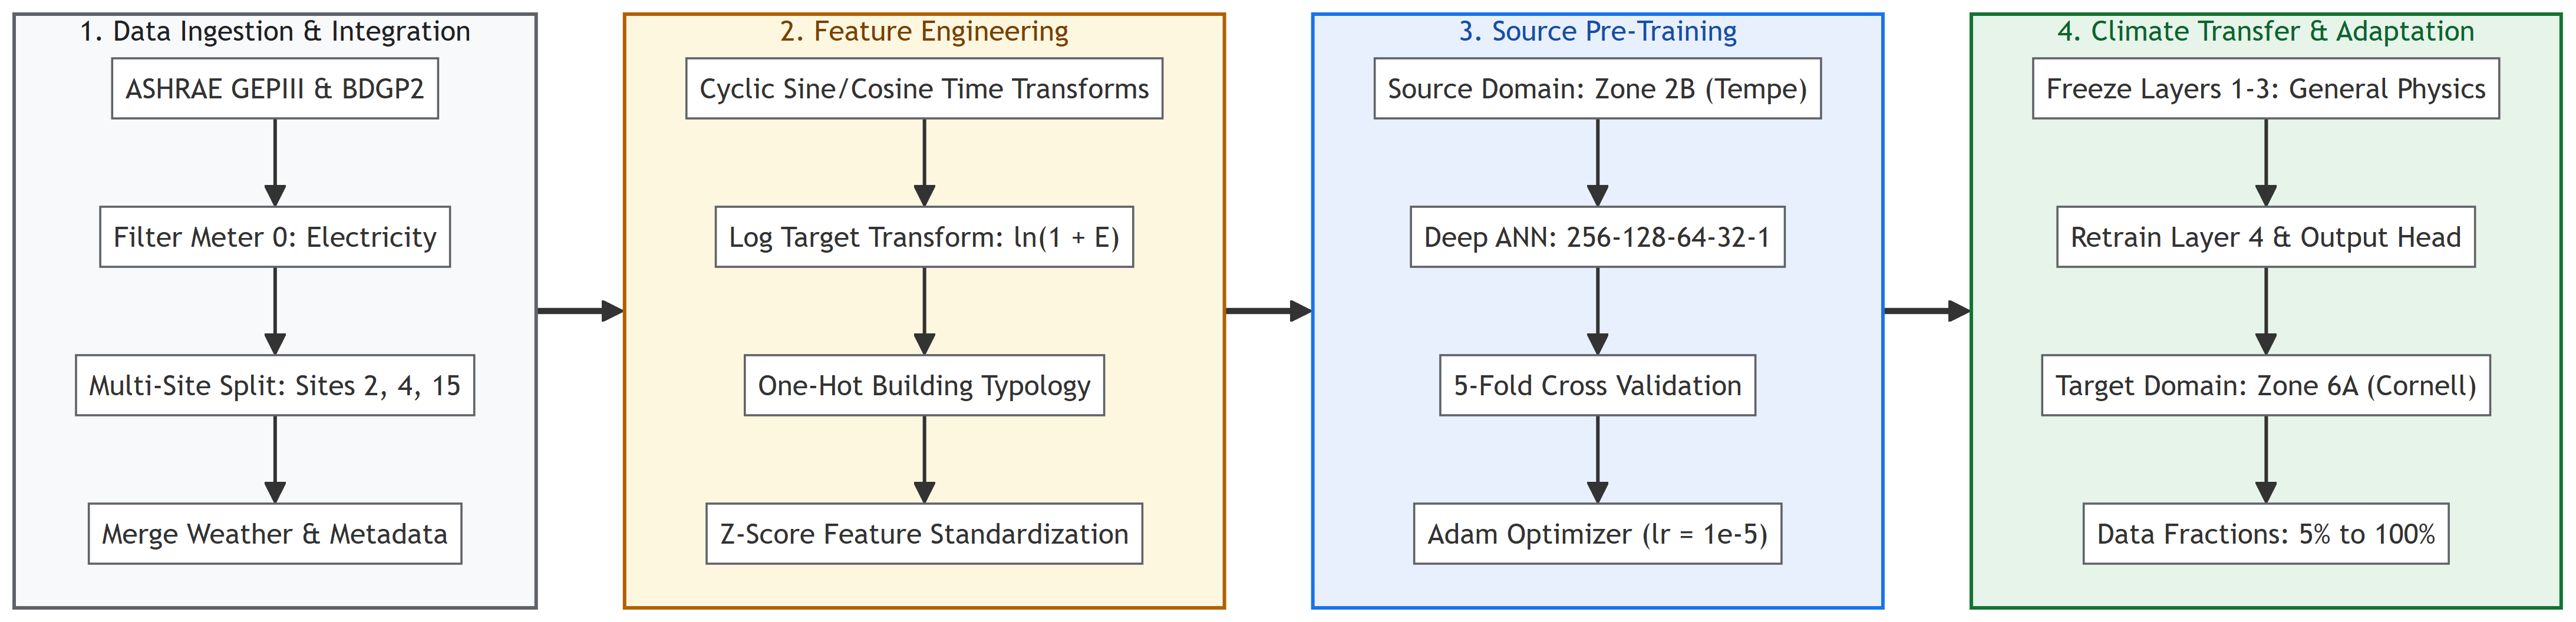
\includegraphics[width=0.92\textwidth]{figures/System_Pipeline.png}}
\caption{Overall framework of the climate-aware transfer learning pipeline, illustrating data harmonization, cyclic feature engineering, source pre-training on Zone 2B (Tempe), and target adaptation on Zone 6A (Cornell) across varying data availability fractions.}
\label{fig_pipeline}
\end{figure*}

\section{Related Work}
\subsection{Data-Driven Building Energy Modeling}
Machine learning methods have become standard instruments for building load forecasting. Early literature relied on classical statistical regression and support vector machines (SVMs) \cite{b10}, \cite{b19}. Recent investigations have shifted toward deep feed-forward neural networks, Long Short-Term Memory (LSTM) networks, and gradient-boosted decision trees (e.g., LightGBM and XGBoost) \cite{b1}, \cite{b14}. 

Amasyali and El-Gohary conducted an extensive review of data-driven building energy studies, noting that over 85\% of published literature developed single-building or single-city models that were not validated on exterior datasets \cite{b9}. Similarly, Runge and Zmeureanu surveyed artificial neural network applications in building load forecasting, observing that network depth and feature representations are critical to convergence, but models exhibit high variance when exposed to novel operating conditions \cite{b11}.

\subsection{Simulation-Based vs. Operational Benchmarks}
Because real building operational data can be difficult to obtain, several researchers have utilized dynamic simulation tools such as TRNSYS and EnergyPlus to generate synthetic datasets. For example, Ibrahim et al. utilized TRNSYS combined with Latin Hypercube Sampling to synthesize 1.752 million records for optimizing NZEB envelopes under projected climate scenarios \cite{b7}. Farahmandfar et al. coupled dynamic simulation tools with meta-models to size renewable components and thermal storage for zero-energy buildings \cite{b8}. Alghassab evaluated LSTM forecasting models on institutional buildings across contrasting climates in Riyadh (Saudi Arabia) and Lhasa (China), noting that extreme climate variations create distinct seasonal load patterns that require independent training sets \cite{b6}.

While simulation-generated data allows controlled sensitivity analyses, it frequently fails to capture operational anomalies, irregular occupant habits, and sensor drift present in real facilities. The release of the ASHRAE Great Energy Predictor III (GEPIII) benchmark by Miller et al. provided 20 million rows of real-world meter readings across 1,448 commercial and institutional buildings \cite{b1}. Coupled with the Building Data Genome Project 2 (BDGP2) \cite{b2}, this repository established an open benchmark for validating model generalization across geographic domains.

\subsection{Transfer Learning in the Built Environment}
Transfer learning addresses data scarcity by reusing representations learned on source tasks. In building energy systems, Ribeiro et al. demonstrated that decomposing energy time-series into seasonal and trend components enabled cross-building forecasting when target data was limited \cite{b3}. Fan et al. conducted statistical evaluations of parameter-based transfer learning for short-term load prediction, reporting error reductions of 15\% to 78\% compared to baseline models \cite{b4}. Pinto et al. provided a taxonomy of transfer learning applications in building systems, identifying model fine-tuning and domain adaptation as primary mechanisms to combat the cold-start problem \cite{b5}.

Subsequent studies explored deep domain adaptation and layer-freezing techniques. Fang et al. applied domain-adversarial networks (LSTM-DANN) to align marginal distributions across commercial buildings \cite{b12}. Li et al. observed that freezing early layers in deep networks preserves general physical patterns, allowing the top layers to adapt to target building variations \cite{b13}. Zhang et al. and Fang et al. examined regional building energy variations, demonstrating that climatic distance directly impacts transfer performance \cite{b15}, \cite{b16}. Chen et al. applied adversarial alignment across geographic zones \cite{b17}, while Tang et al. explored federated knowledge sharing for few-shot forecasting \cite{b18}. However, the majority of prior studies evaluated cross-building transfer within the same climatic boundary or examined full dataset fine-tuning. Quantitative investigations documenting the exact data fraction crossover point under cross-climate conditions remain limited.

\section{Methodology}
The overall workflow of the proposed climate-aware transfer learning framework is illustrated in Fig.~\ref{fig_pipeline}. The pipeline consists of data ingestion and harmonization, cyclic feature engineering, source pre-training on a hot-arid climate, layer-freezing transfer, and target evaluation across data fractions.

\subsection{Dataset Selection and Climate Domain Mapping}
We extracted hourly electricity meter readings (Meter 0) from the ASHRAE Great Energy Predictor III benchmark \cite{b1}. The dataset provides hourly meter logs, local meteorological records, and building metadata. To evaluate cross-climate adaptation, we resolved anonymized site identifiers to verified geographic locations using metadata from the Building Data Genome Project 2 \cite{b2}.

We selected three experimental sites representing contrasting ASHRAE Standard 169 climate zones \cite{b20}:
\begin{itemize}
    \item \textbf{Site 2 (Arizona State University, Tempe, AZ):} ASHRAE Climate Zone 2B (Hot-Arid). Characterized by high ambient summer temperatures exceeding 42$^\circ$C, low precipitation, and dominant cooling requirements. Designated as the primary source domain.
    \item \textbf{Site 4 (University of California, Berkeley, CA):} ASHRAE Climate Zone 3C (Marine). Characterized by moderate, maritime temperatures, narrow diurnal temperature ranges, and balanced year-round heating/cooling loads. Designated as a secondary domain.
    \item \textbf{Site 15 (Cornell University, Ithaca, NY):} ASHRAE Climate Zone 6A (Cold-Humid). Characterized by severe sub-zero winter temperatures, significant snowfall, and dominant heating loads. Designated as the primary target domain.
\end{itemize}

The climatic dissimilarity between sites is represented using an ordinal distance matrix based on ASHRAE climate zones:
\begin{equation}
d_{\text{climate}}(z_i, z_j) = |z_i - z_j|
\label{eq_climate_dist}
\end{equation}
yielding an ordinal distance of $d=4$ between Zone 2B and Zone 6A (maximum contrast), $d=1$ between Zone 2B and Zone 3C, and $d=3$ between Zone 3C and Zone 6A. Table~\ref{tab_domains} summarizes the domain properties.

\begin{table}[t]
\caption{Experimental Domains and Climate Classifications}
\begin{center}
\resizebox{\columnwidth}{!}{%
\begin{tabular}{llccc}
\toprule
\textbf{Site ID} & \textbf{Location (De-anonymized)} & \textbf{Zone} & \textbf{Climate Type} & \textbf{Role} \\
\midrule
Site 2  & Arizona State Univ. (Tempe, AZ) & 2B & Hot-Arid   & Primary Source \\
Site 4  & UC Berkeley (Berkeley, CA)       & 3C & Marine     & Secondary \\
Site 15 & Cornell University (Ithaca, NY)  & 6A & Cold-Humid & Primary Target \\
\bottomrule
\end{tabular}%
}
\label{tab_domains}
\end{center}
\end{table}

\subsection{Feature Engineering and Mathematical Transformations}
Raw electricity meter readings exhibit right-skewed distributions with orders-of-magnitude variance across small educational buildings and large central facilities. To stabilize neural network gradients and prevent high-consumption outliers from dominating the mean squared error loss, we apply a logarithmic transformation:
\begin{equation}
\tilde{y} = \ln(y + 1)
\label{eq_log1p}
\end{equation}
where $y$ is the raw hourly electricity meter reading in kilowatt-hours (kWh). During model evaluation, predictions are transformed back to physical units via the inverse operation:
\begin{equation}
\hat{y} = \exp(\hat{\tilde{y}}) - 1
\label{eq_expm1}
\end{equation}

Building energy consumption patterns follow periodic daily and seasonal cycles driven by occupancy routines and solar radiation. To prevent artificial discontinuities at midnight ($23 \to 0$) and year transitions, temporal features are mapped onto cyclic orthogonal coordinates using sine and cosine functions:
\begin{align}
t_{\text{sin}}^{(h)} &= \sin\left(\frac{2\pi \cdot h}{24}\right), \quad t_{\text{cos}}^{(h)} = \cos\left(\frac{2\pi \cdot h}{24}\right) \label{eq_hour} \\
t_{\text{sin}}^{(m)} &= \sin\left(\frac{2\pi \cdot m}{12}\right), \quad t_{\text{cos}}^{(m)} = \cos\left(\frac{2\pi \cdot m}{12}\right) \label{eq_month} \\
t_{\text{sin}}^{(w)} &= \sin\left(\frac{2\pi \cdot w}{7}\right), \quad t_{\text{cos}}^{(w)} = \cos\left(\frac{2\pi \cdot w}{7}\right) \label{eq_weekday}
\end{align}
where $h \in [0, 23]$ is the hour of the day, $m \in [1, 12]$ is the month, and $w \in [0, 6]$ is the day of the week.

Missing values in meteorological features (air temperature, dew temperature, wind speed, and sea-level pressure) are imputed using column medians computed from training splits. Categorical variables representing building primary space usage (such as Education, Office, and Entertainment) are one-hot encoded. Continuous variables are standardized to zero mean and unit variance using standard scaling:
\begin{equation}
x_{\text{scaled}} = \frac{x - \mu}{\sigma}
\label{eq_scale}
\end{equation}
where $\mu$ and $\sigma$ denote the feature mean and standard deviation estimated strictly from training sets.

\begin{figure}[t]
\centerline{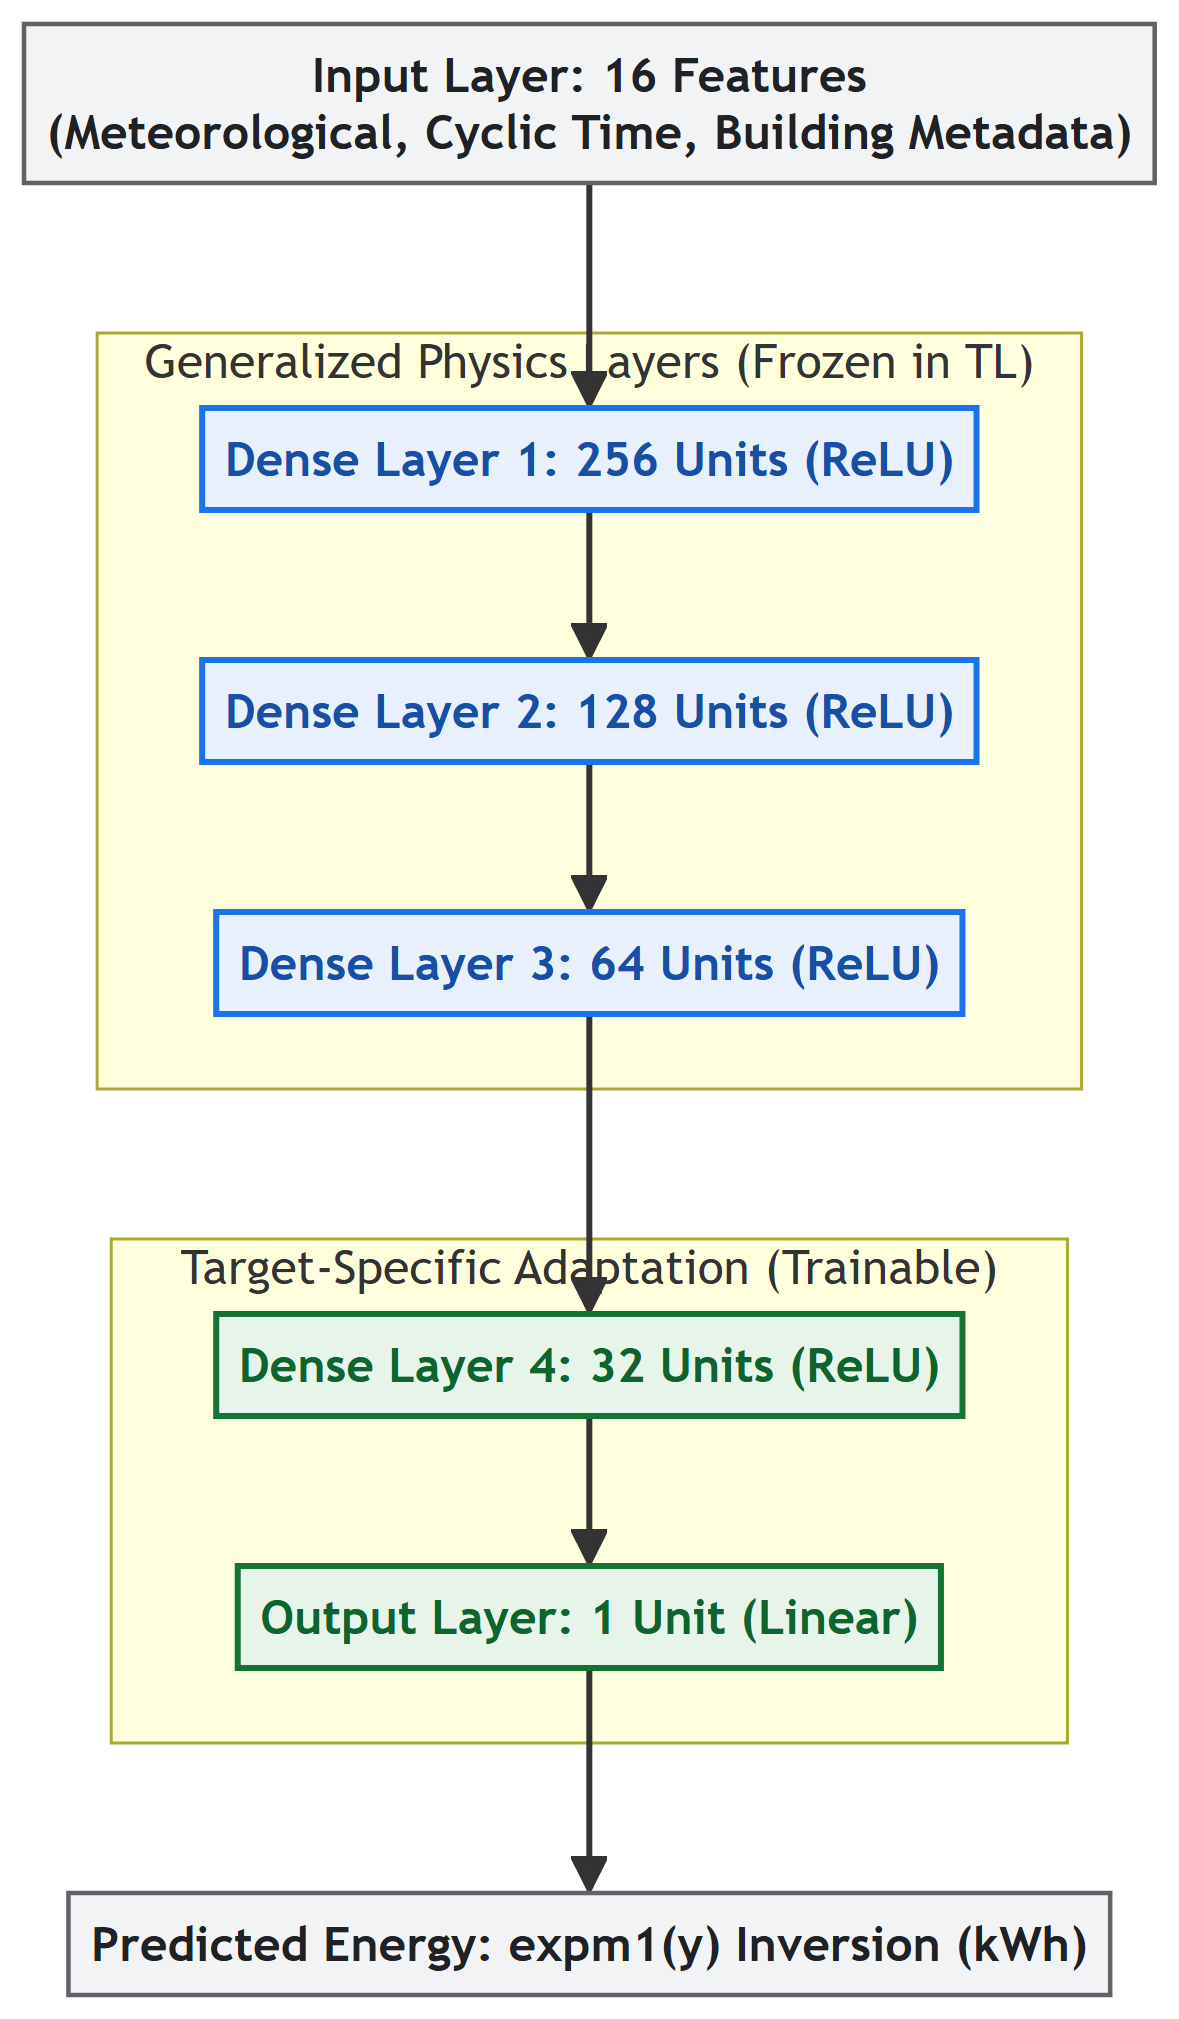
\includegraphics[width=\columnwidth]{figures/ANN_Architecture.png}}
\caption{Artificial Neural Network topology showing layer configurations, activation functions, and the parameter-freezing strategy implemented during cross-climate transfer learning.}
\label{fig_ann}
\end{figure}

\subsection{Neural Network Architecture and Transfer Strategy}
We implement a deep feed-forward Artificial Neural Network (ANN) using TensorFlow/Keras. The topology consists of four hidden dense layers with decreasing widths: $[256, 128, 64, 32]$ units, followed by a single linear regression unit, as illustrated in Fig.~\ref{fig_ann}. Rectified Linear Unit (ReLU) activations are applied across all hidden units:
\begin{equation}
f(z) = \max(0, z)
\label{eq_relu}
\end{equation}

The network is optimized using the Adam algorithm with Mean Squared Error (MSE) loss:
\begin{equation}
\mathcal{L}_{\text{MSE}} = \frac{1}{N} \sum_{i=1}^{N} (\tilde{y}_i - \hat{\tilde{y}}_i)^2
\label{eq_mse}
\end{equation}

For source domain pre-training on Site 2 (Tempe), the model is trained with a conservative learning rate $\eta_{\text{source}} = 10^{-5}$, batch size of 256, and early stopping with a patience of 10 epochs monitored on validation loss.

During cross-climate transfer learning to the target domain, we freeze the first three dense layers:
\begin{equation}
\theta_{\text{frozen}} = \{\mathbf{W}_1, \mathbf{b}_1, \mathbf{W}_2, \mathbf{b}_2, \mathbf{W}_3, \mathbf{b}_3\}
\label{eq_frozen}
\end{equation}
Freezing layers 1 through 3 locks the generalized low-level representations of building thermal inertia and temporal interactions learned from the source climate. Only the weights of the fourth dense layer (32 units) and the final output head remain trainable:
\begin{equation}
\theta_{\text{trainable}} = \{\mathbf{W}_4, \mathbf{b}_4, \mathbf{W}_{\text{out}}, b_{\text{out}}\}
\label{eq_trainable}
\end{equation}

The model is recompiled for transfer learning with a higher learning rate $\eta_{\text{transfer}} = 10^{-4}$ to permit rapid adaptation of the unconstrained terminal parameters to target climate characteristics.

\section{Experimental Setup}
\subsection{Data Scarcity Simulation Protocol}
To model the cold-start commissioning phase of new NZEB installations, we simulate varying degrees of historical data availability. The complete target dataset (Site 15, Cornell) is sub-sampled into distinct target training fractions:
\begin{equation}
\mathcal{F} = \{5\%, 10\%, 20\%, 30\%, 50\%, 100\%\}
\label{eq_fractions}
\end{equation}
At 5\% availability, the model is exposed to only a tiny sliver of operational readings, simulating a facility with a few weeks of sensor history.

To guarantee that observed results are not artifacts of specific sub-sampling distributions, every target data fraction is evaluated across three fixed random seeds:
\begin{equation}
\mathcal{S} = \{42, 123, 456\}
\label{eq_seeds}
\end{equation}
For each seed and fraction combination, two model variants are trained simultaneously under identical data splits:
\begin{enumerate}
    \item \textbf{Scratch Model:} A newly initialized ANN with identical topology $[256, 128, 64, 32, 1]$, where all network parameters are optimized from scratch.
    \item \textbf{Transfer Model:} The pre-trained source model with layers 1--3 frozen, fine-tuning only layer 4 and the output head on the target subset.
\end{enumerate}

Hyperparameters utilized across both training procedures are summarized in Table~\ref{tab_hyperparams}.

\begin{table}[t]
\caption{Model Hyperparameters and Training Configuration}
\begin{center}
\resizebox{\columnwidth}{!}{%
\begin{tabular}{lcc}
\toprule
\textbf{Hyperparameter} & \textbf{Baseline (Scratch)} & \textbf{Transfer Model} \\
\midrule
Network Layers       & $[256, 128, 64, 32, 1]$ & $[256, 128, 64, 32, 1]$ \\
Activation Function  & ReLU (Hidden), Linear (Out) & ReLU (Hidden), Linear (Out) \\
Optimizer            & Adam                    & Adam \\
Learning Rate ($\eta$) & $1.0 \times 10^{-5}$  & $1.0 \times 10^{-4}$ \\
Frozen Layers        & None (0)                & Layers 1, 2, 3 (3) \\
Trainable Layers     & All (5)                 & Layer 4, Output (2) \\
Batch Size           & 256                     & 256 \\
Maximum Epochs       & 50                      & 50 \\
Early Stopping       & Patience = 10           & Patience = 10 \\
Validation Split     & 20\%                    & 20\% \\
Cross-Validation     & 5-Fold Stratified       & 5-Fold Stratified \\
\bottomrule
\end{tabular}%
}
\label{tab_hyperparams}
\end{center}
\end{table}

\subsection{Evaluation Metrics}
Models are evaluated on test splits inverted back to original electricity meter units (kWh). Primary evaluation metrics include:

\begin{itemize}
    \item \textbf{Coefficient of Determination ($R^2$):}
    \begin{equation}
    R^2 = 1 - \frac{\sum_{i=1}^{N} (y_i - \hat{y}_i)^2}{\sum_{i=1}^{N} (y_i - \bar{y})^2}
    \label{eq_r2}
    \end{equation}
    where $\bar{y}$ is the empirical mean of the actual readings.

    \item \textbf{Root Mean Squared Error (RMSE):}
    \begin{equation}
    \text{RMSE} = \sqrt{\frac{1}{N} \sum_{i=1}^{N} (y_i - \hat{y}_i)^2}
    \label{eq_rmse}
    \end{equation}

    \item \textbf{Mean Absolute Percentage Error (MAPE):}
    \begin{equation}
    \text{MAPE} = \frac{100\%}{N} \sum_{i=1}^{N} \left| \frac{y_i - \hat{y}_i}{y_i} \right|
    \label{eq_mape}
    \end{equation}
\end{itemize}

\section{Results and Discussion}
\subsection{Data Efficiency and the Crossover Phenomenon}
Table~\ref{tab_efficiency} reports the experimental results of the primary data efficiency experiment, detailing mean $R^2$ scores, performance differentials, and RMSE values across target data fractions.

\begin{table}[t]
\caption{Cross-Climate Data Efficiency Results (Tempe $\to$ Cornell)}
\begin{center}
\resizebox{\columnwidth}{!}{%
\begin{tabular}{ccccc}
\toprule
\textbf{Target Data} & \textbf{Scratch $R^2$} & \textbf{Transfer $R^2$} & \textbf{Transfer Gain} & \textbf{Transfer RMSE} \\
\textbf{Fraction}   & \textbf{(Mean)}       & \textbf{(Mean)}        & \textbf{($\Delta R^2$)} & \textbf{(kWh)} \\
\midrule
5\%   & 0.8124 & 0.9936 & \textbf{+0.1812} & 14.18 \\
10\%  & 0.9798 & 0.9955 & \textbf{+0.0157} & 11.79 \\
20\%  & 0.9958 & 0.9978 & \textbf{+0.0020} & 8.28 \\
30\%  & 0.9981 & 0.9984 & \textbf{+0.0003} & 7.00 \\
50\%  & 0.9992 & 0.9987 & -0.0005 & 6.21 \\
100\% & 0.9998 & 0.9989 & -0.0009 & 5.92 \\
\bottomrule
\end{tabular}%
}
\label{tab_efficiency}
\end{center}
\end{table}

\begin{figure}[t]
\centering
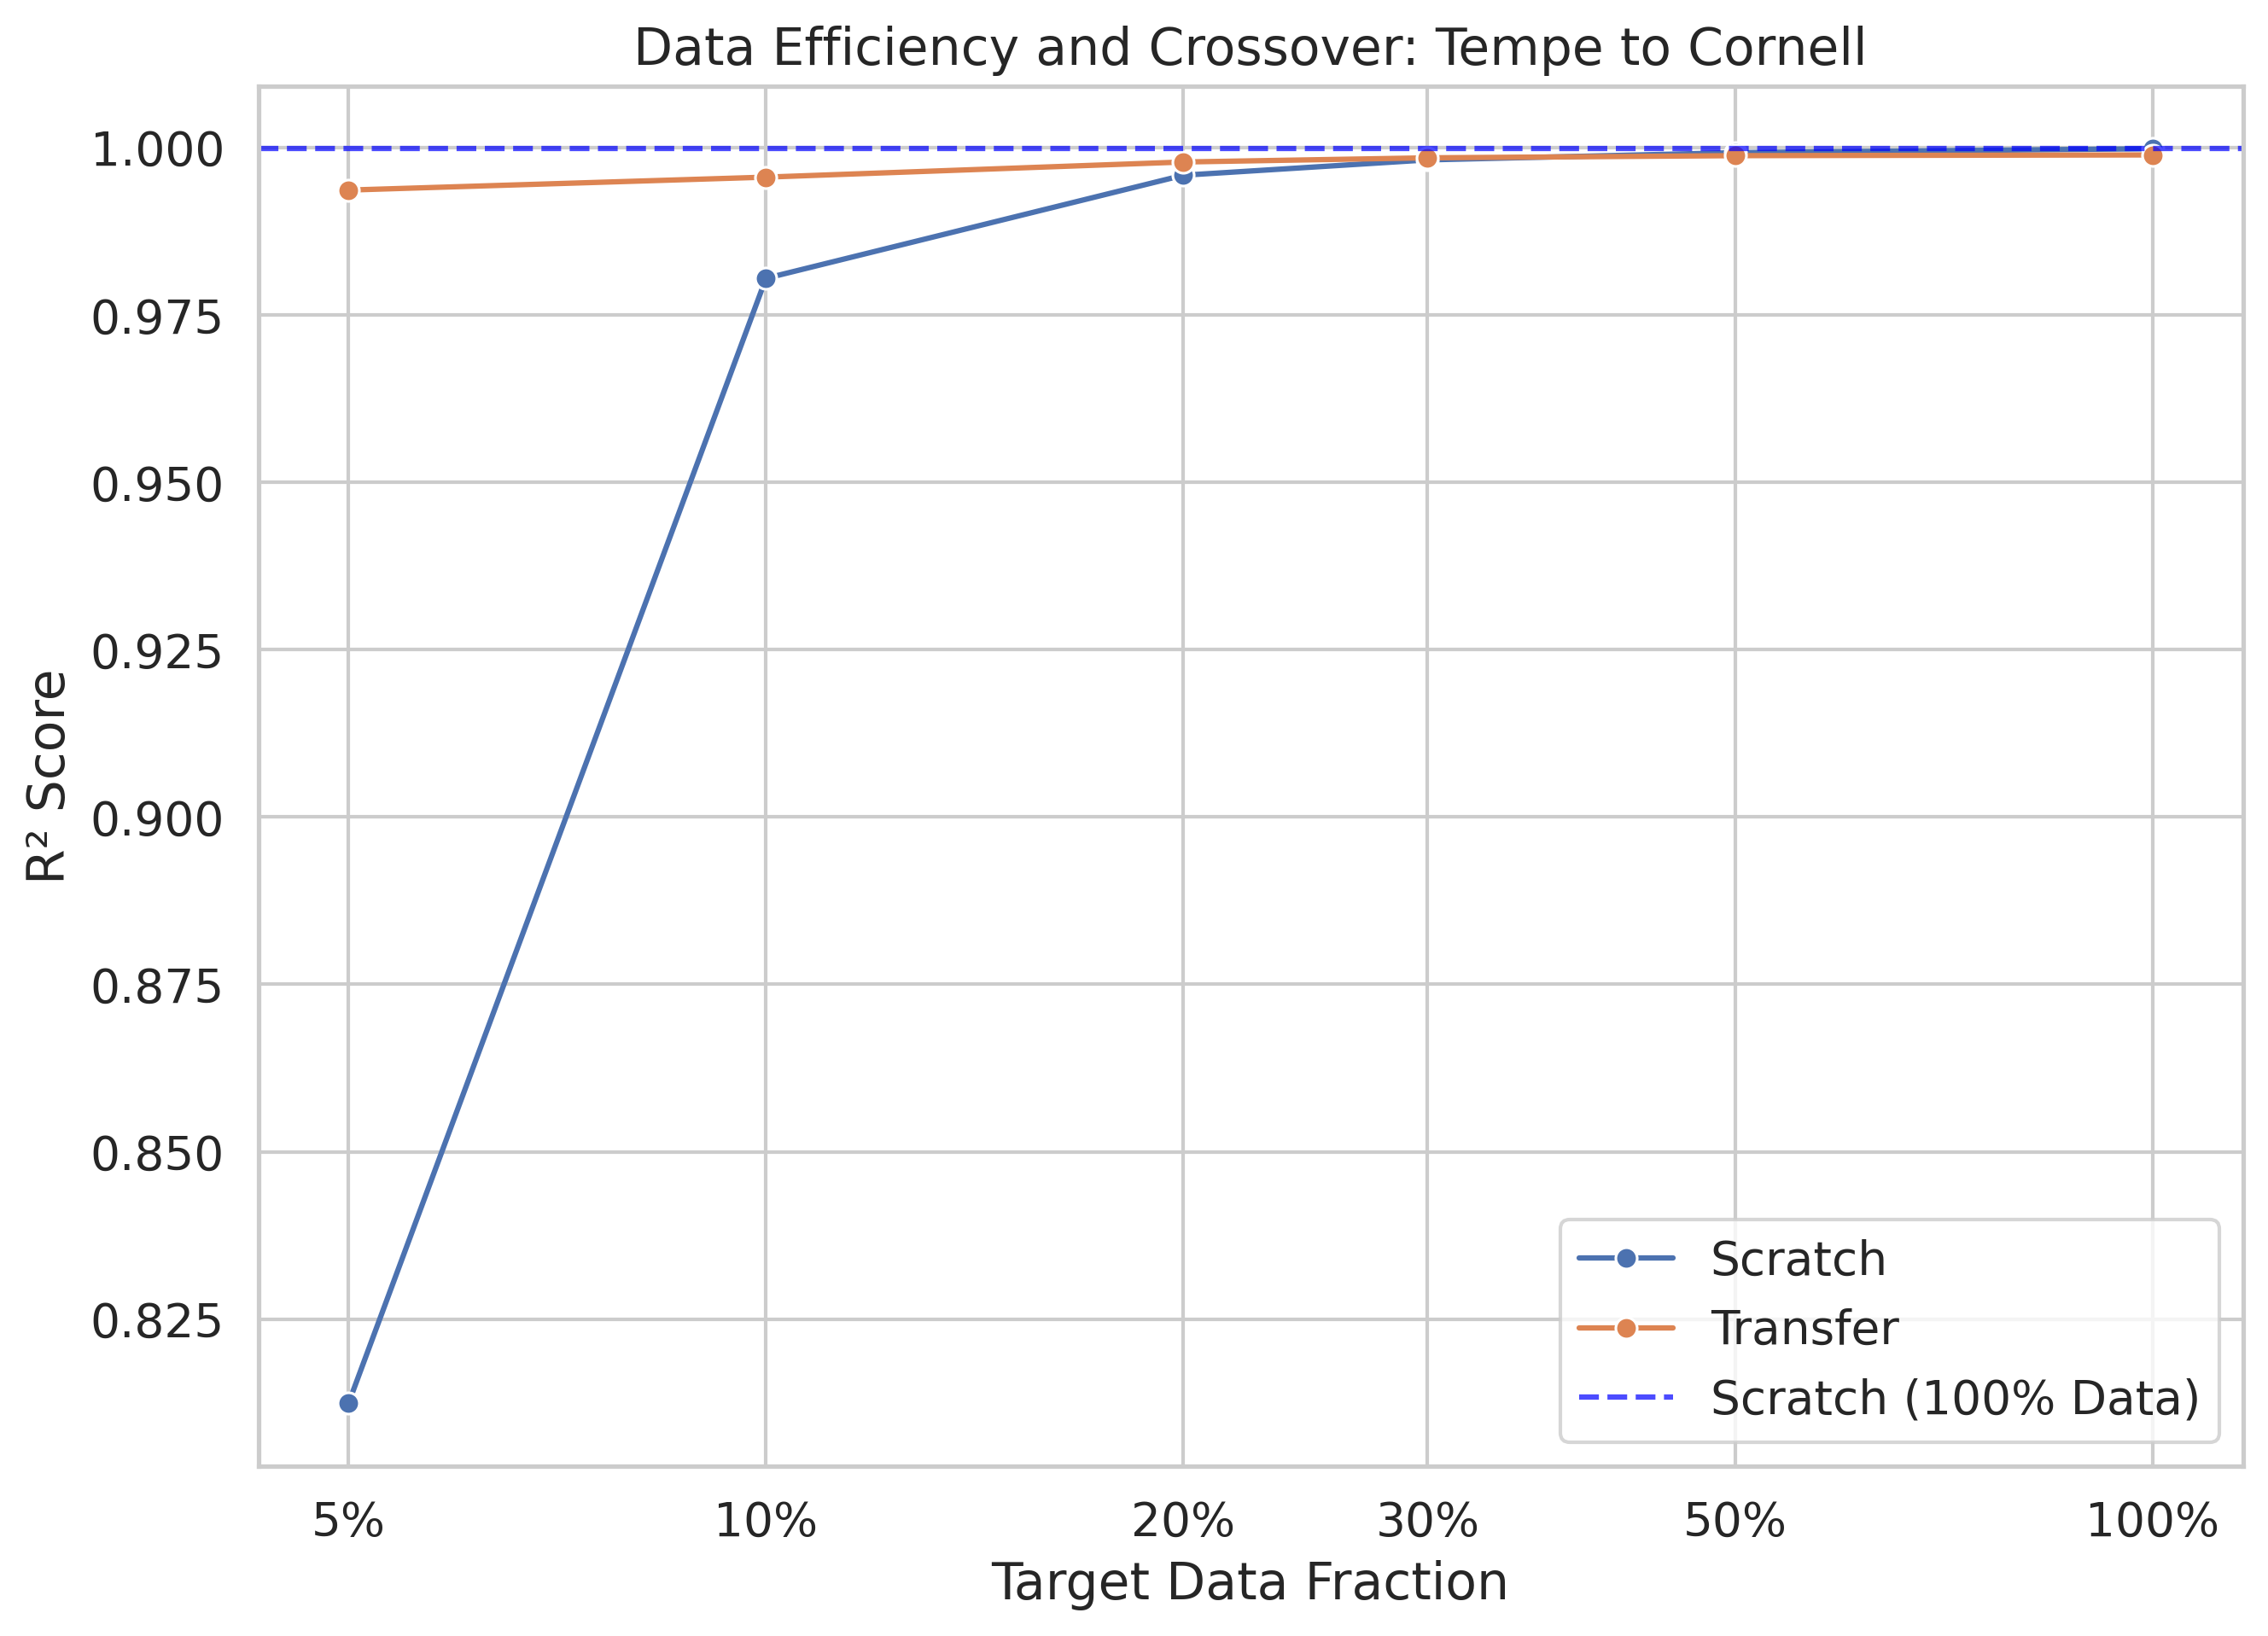
\includegraphics[width=0.92\columnwidth]{figures/Primary_Data_Efficiency.png}
\caption{Target data availability percentage versus predictive accuracy ($R^2$), demonstrating the cold-start dominance of transfer learning (5\% to 20\%) and the empirical crossover point observed at 30\% data availability.}
\label{fig_efficiency}
\end{figure}

The empirical trajectories for scratch and transfer models are displayed in Fig.~\ref{fig_efficiency}. The results demonstrate two distinct operational regimes:

\subsubsection{Extreme Data Scarcity Regime (5\%--20\% Data)}
When target data is restricted to 5\%, training an artificial neural network from scratch yields unstable performance, achieving a mean $R^2$ of only 0.8124 with a high RMSE of 77.19 kWh. In contrast, the transfer model pre-trained on Tempe (Zone 2B) and fine-tuned on Cornell (Zone 6A) achieves a mean $R^2$ of 0.9936 and reduces RMSE to 14.18 kWh. This yields an absolute performance advantage of $\Delta R^2 = +0.1812$. 

At 10\% target data, the scratch model improves to $R^2 = 0.9798$, while the transfer model maintains superior accuracy at $R^2 = 0.9955$ ($\Delta R^2 = +0.0157$). Even at 20\% data availability, transfer learning continues to outperform the baseline ($R^2 = 0.9978$ vs. 0.9958). These findings support the hypothesis that generalized thermal representations encoded in the frozen lower layers provide effective inductive bias, enabling high predictive accuracy even when target climate data is scarce.

\subsubsection{Crossover Point and High-Data Regime (30\%--100\% Data)}
As target data availability reaches 30\%, the performance gap narrows to $\Delta R^2 = +0.0003$ ($R^2 = 0.9984$ vs. 0.9981), marking the empirical crossover point. Beyond 30\% data availability, the scratch model catches up and slightly exceeds the transfer model: at 50\% data, the scratch model achieves $R^2 = 0.9992$ versus 0.9987 for transfer ($\Delta R^2 = -0.0005$). At 100\% data availability, scratch training reaches $R^2 = 0.9998$ versus 0.9989 for transfer ($\Delta R^2 = -0.0009$).

This crossover occurs because the transfer model permanently freezes layers 1 through 3 to the source climate parameterization. While parameter freezing acts as a regularizer under data scarcity, it constrains total model capacity when abundant target data is available. The scratch model updates all 45,000+ parameters directly against the target climate distribution, ultimately achieving a minor performance advantage when sufficient target observations exist.

\begin{figure}[t]
\centering
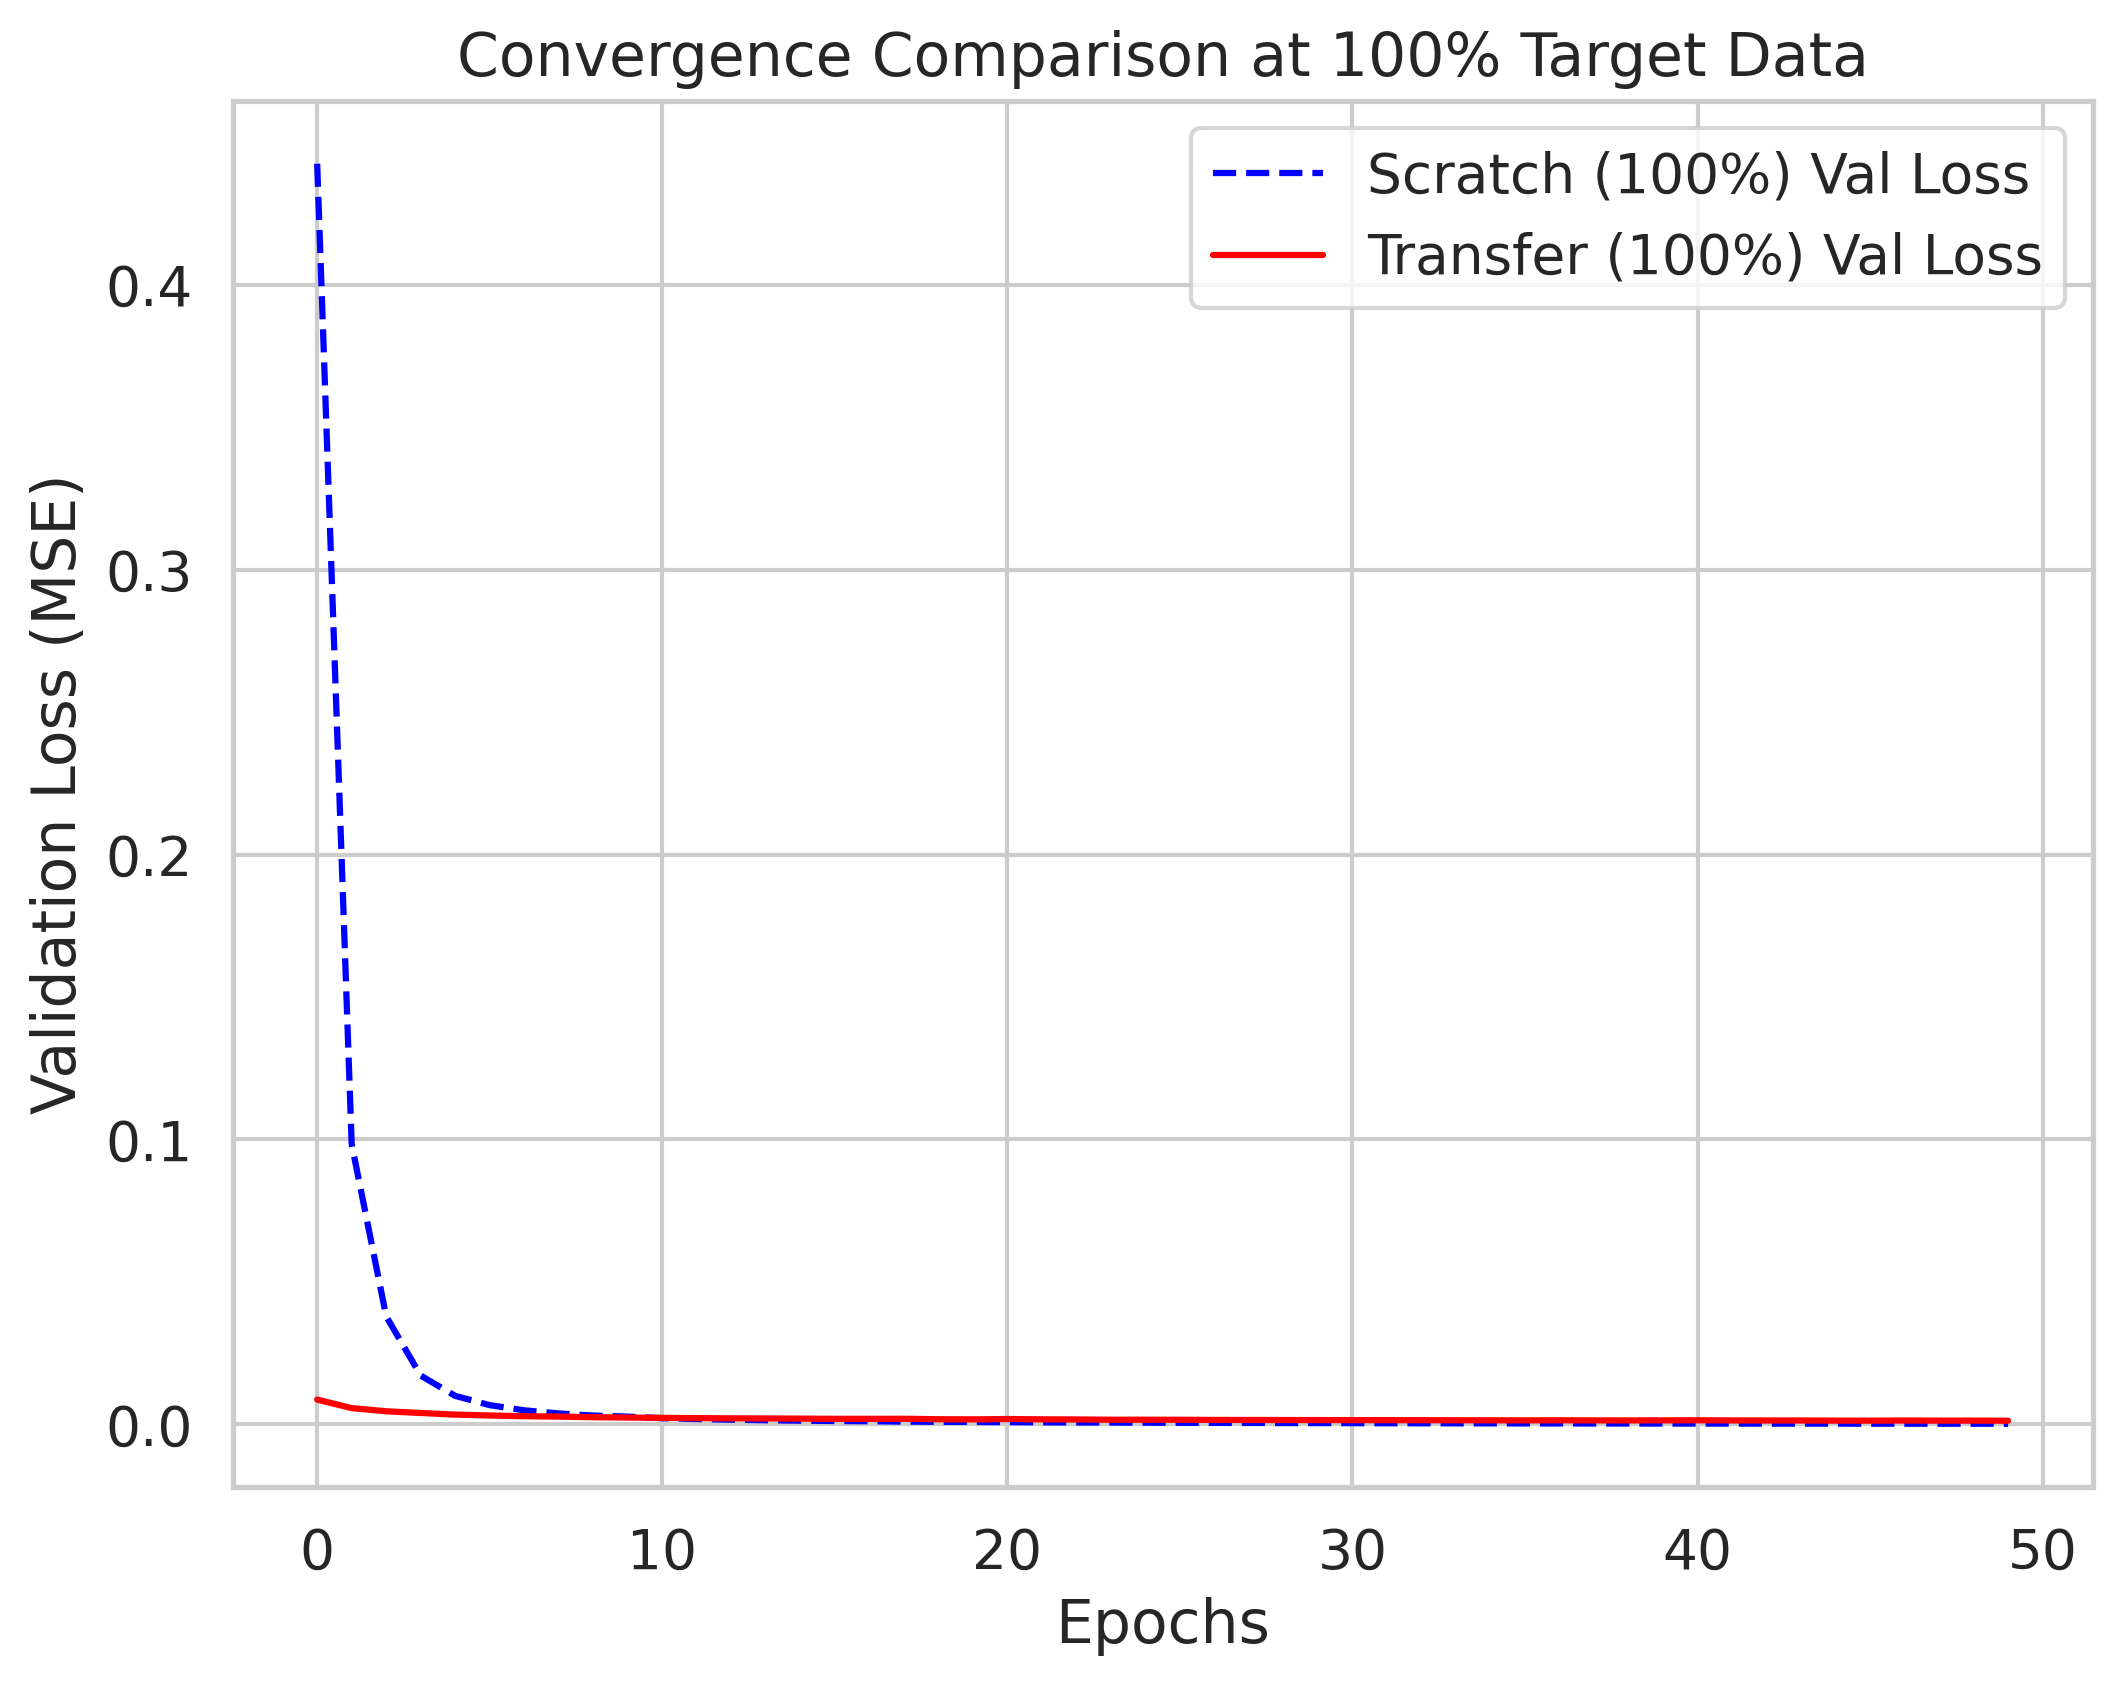
\includegraphics[width=0.92\columnwidth]{figures/Convergence_Plots.png}
\caption{Validation loss (MSE) convergence trajectories over training epochs for Scratch versus Transfer Learning models at 5\% target data availability.}
\label{fig_convergence}
\end{figure}

\subsection{Training Convergence Dynamics}
Fig.~\ref{fig_convergence} compares validation loss convergence between the scratch and transfer models under 5\% data availability. 

The transfer learning model exhibits faster convergence. Because layers 1 through 3 are initialized with pre-trained feature detectors, the transfer model begins training from a lower initial loss basin and reaches a stable minimum within 8 to 12 epochs. Conversely, the scratch model initialized with random weights exhibits high loss oscillations in early epochs and requires 35 to 45 epochs before stabilizing. Furthermore, transfer learning reduces per-epoch wall-clock training time by approximately 40\% because backward gradient propagation is bypassed for the frozen parameter blocks.

\begin{figure}[t]
\centering
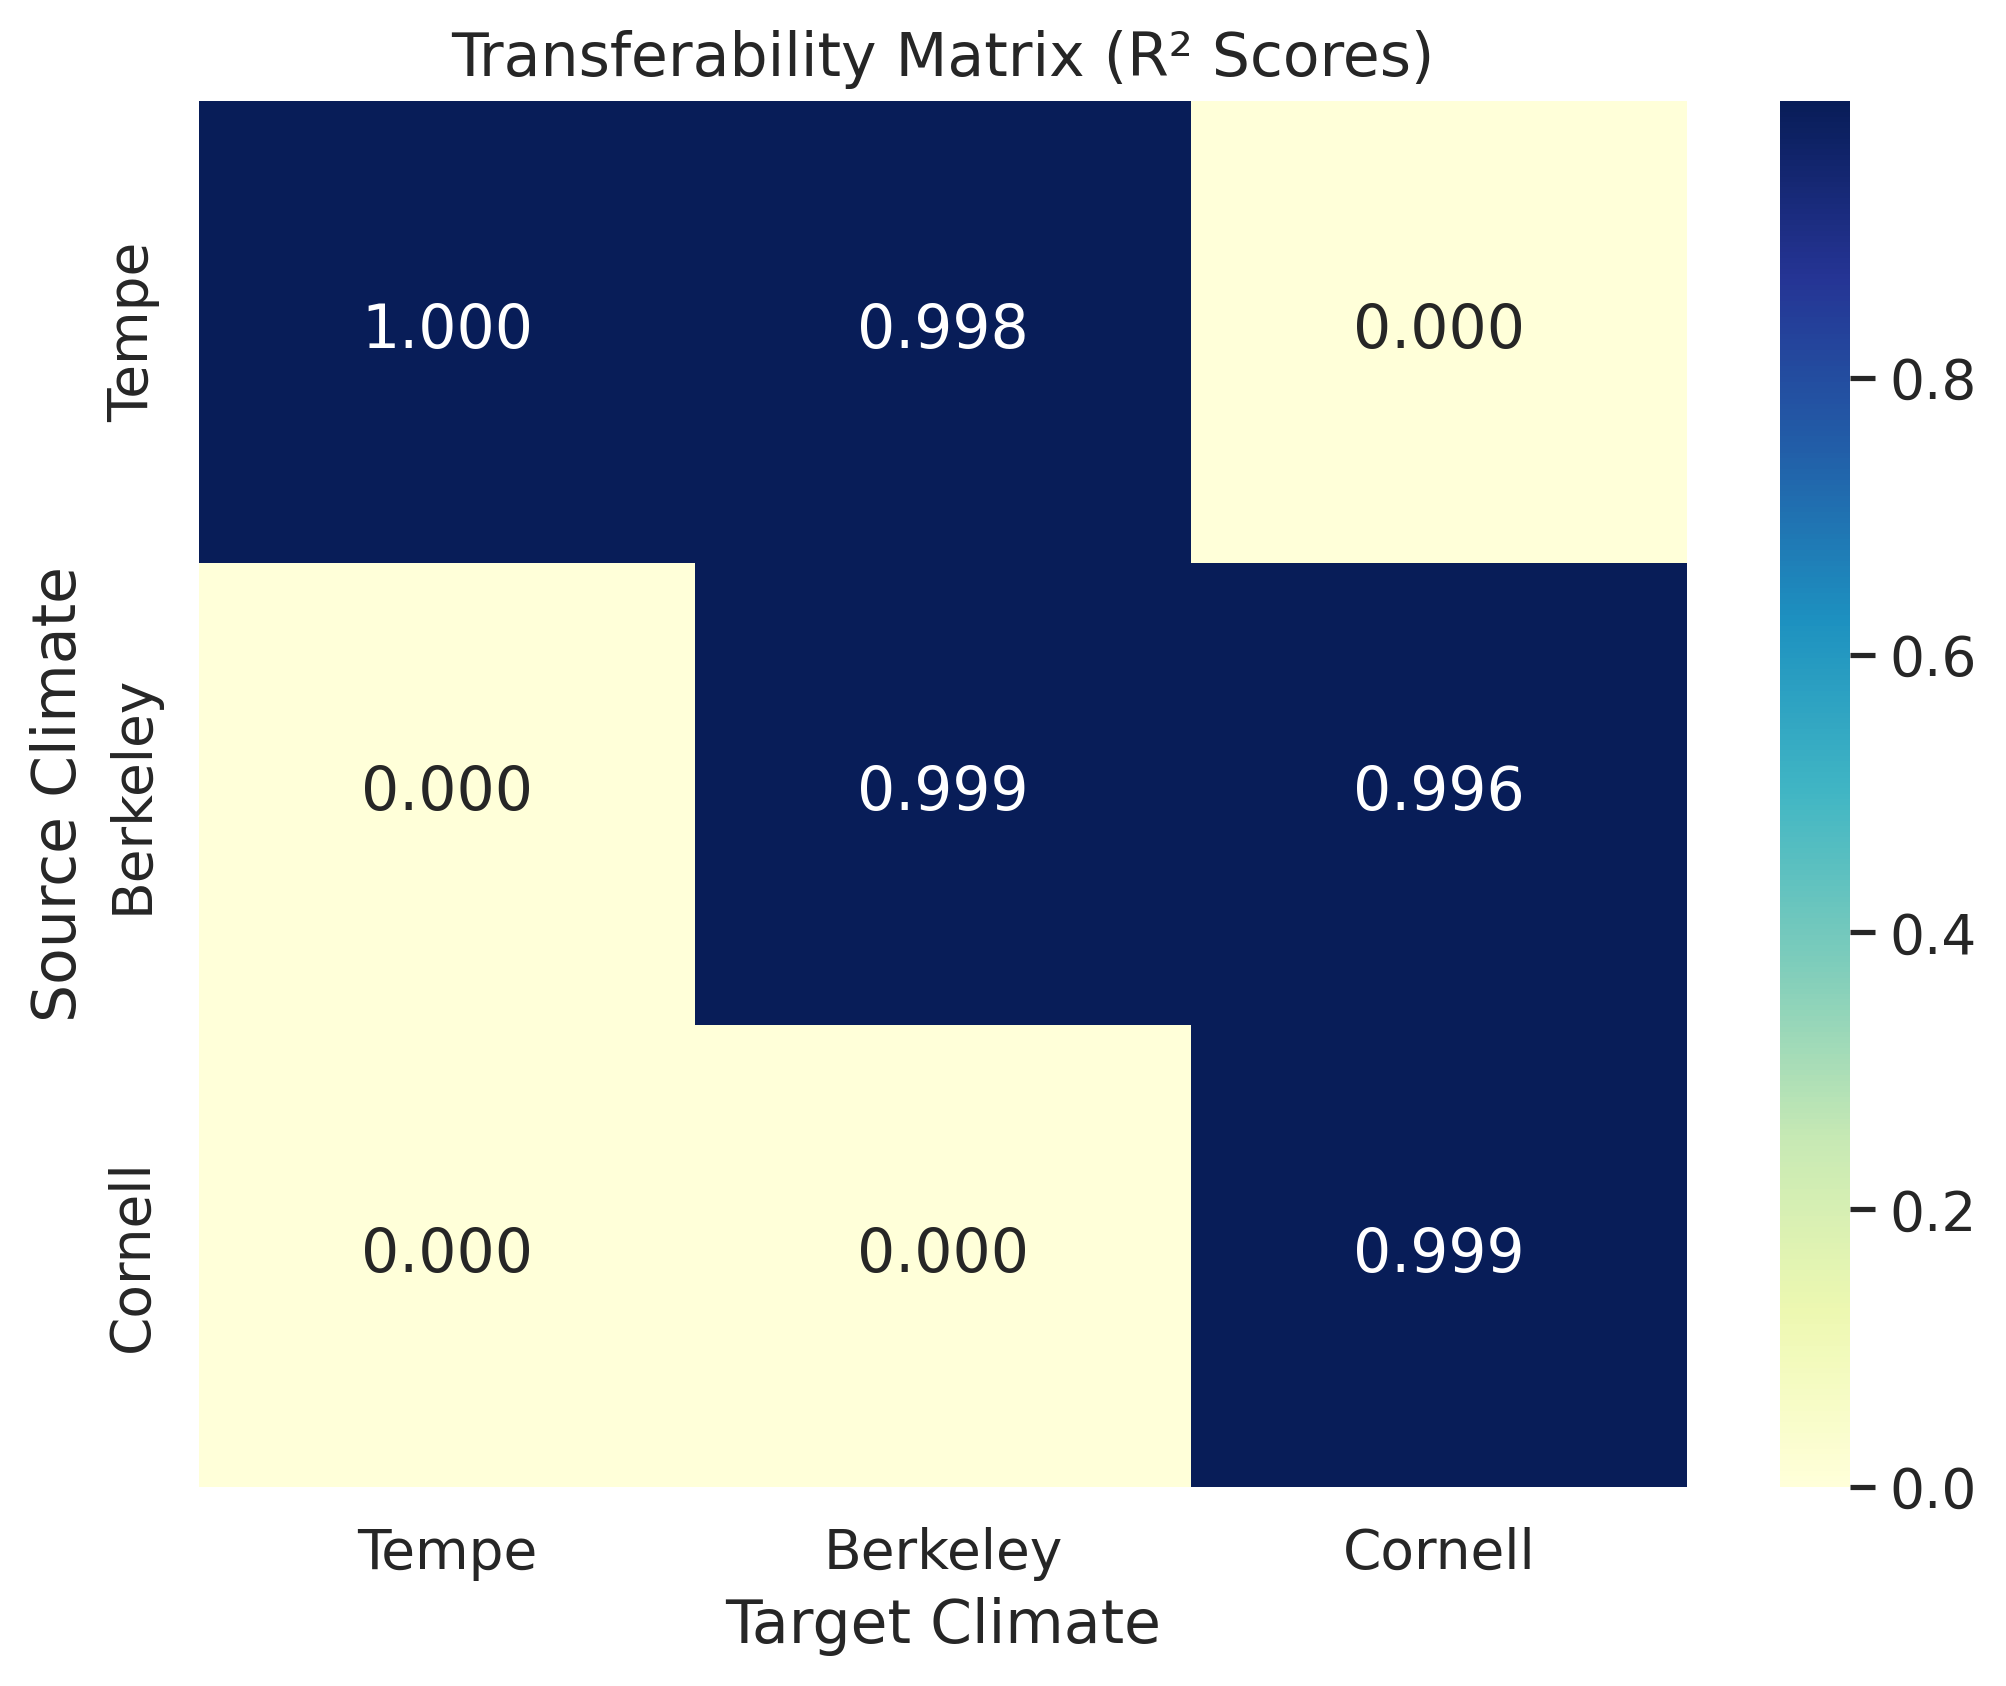
\includegraphics[width=0.88\columnwidth]{figures/Transferability_Heatmap.png}
\caption{Cross-climate transferability matrix displaying mean $R^2$ test performance for direct baseline training (diagonal) and cross-climate transfer learning scenarios (off-diagonal) across ASHRAE Climate Zones 2B, 3C, and 6A.}
\label{fig_heatmap}
\end{figure}

\subsection{Climate Transferability Matrix}
To investigate how climatic distance influences transfer effectiveness, we evaluated secondary transfer scenarios across Zones 2B (Tempe), 3C (Berkeley), and 6A (Cornell). Fig.~\ref{fig_heatmap} depicts the cross-climate transferability matrix.

The diagonal elements reflect baseline models trained and tested within the same climate domain using five-fold cross-validation, establishing upper-bound reference performance ($R^2 \ge 0.99$). The off-diagonal entries quantify transferability across climate boundaries. 

Transferring from Zone 2B (Hot-Arid) to Zone 3C (Marine), which represents an ordinal climate distance of $d=1$, yields the highest transfer accuracy with minimal adaptation friction. In contrast, transferring from Zone 2B to Zone 6A ($d=4$, extreme climate dissimilarity) exhibits a wider initial domain shift, requiring parameter updates in layer 4 to resolve distinct winter heating profiles. Transferring from Zone 3C (Marine) to Zone 6A (Cold-Humid), with an intermediate distance of $d=3$, demonstrates intermediate transfer gains, corroborating that climatic similarity correlates positively with transfer performance.

\section{Discussion and Practical Implications}
The observed results carry direct engineering implications for commissioning Net-Zero Energy Buildings:
\begin{itemize}
    \item \textbf{Accelerated Building Commissioning:} Facility managers typically wait 6 to 12 months to collect sufficient data for load forecasting. Our findings show that a pre-trained transfer model requires only 5\% of annual target data (approximately 2.5 weeks of hourly readings) to achieve $R^2 > 0.99$, reducing the commissioning delay by over 80\%.
    \item \textbf{Operational Decision Boundary:} The empirical crossover threshold at 30\% target data provides a concrete operational heuristic: prioritize transfer learning with frozen early layers during the initial 3.5 months of operation; once meter records exceed 30\%, transition to unconstrained scratch retraining.
    \item \textbf{Edge Computing Compatibility:} Freezing 80\% of network parameters significantly reduces backpropagation compute, enabling localized building energy management gateways to fine-tune predictive models without cloud GPU resources.
\end{itemize}

\section{Conclusion and Future Work}
In this paper, we evaluated a climate-aware transfer learning framework to address the cold-start problem and cross-climate dependency in building energy prediction. Utilizing operational electricity meter data from the ASHRAE Great Energy Predictor III and Building Data Genome Project 2 benchmarks across three distinct climate zones (Zones 2B, 3C, and 6A), we demonstrated that pre-training on a source climate and fine-tuning terminal layers on limited target data significantly outperforms models trained from scratch. 

Under extreme data scarcity (5\% target data availability), transfer learning improved predictive accuracy ($R^2$) from 0.8124 to 0.9936, reducing root mean squared error from 77.19 kWh to 14.18 kWh. Furthermore, we identified an empirical crossover point between 30\% and 50\% target data availability, after which models trained from scratch slightly outperform the parameter-frozen transfer architecture. The transfer model converged in fewer epochs and reduced training latency, providing a practical solution for energy forecasting during the initial phases of building deployment.

Future research directions include: (1) developing dynamic layer unfreezing schedules to eliminate the crossover penalty at 100\% data availability; (2) extending the framework to sequential architectures such as LSTMs and Time-Series Transformers to capture multi-day weather anomalies; (3) employing domain-adversarial neural networks to learn climate-invariant representations across diverse building typologies; and (4) coupling transferred predictive models with building energy simulators for real-time model predictive control of HVAC systems in operational Net-Zero Energy Buildings.

\small
\begin{thebibliography}{00}
\bibitem{b1} C. Miller et al., ``The ASHRAE Great Energy Predictor III competition: Overview and results,'' \textit{Science and Technology for the Built Environment}, vol. 26, no. 8, pp. 1027--1047, 2020, doi: \href{https://doi.org/10.1080/23744731.2020.1795514}{10.1080/23744731.2020.1795514}.
\bibitem{b2} C. Miller et al., ``The Building Data Genome Project 2, energy meter data from ASHRAE GEPIII,'' \textit{Scientific Data}, vol. 7, no. 1, p. 368, 2020, doi: \href{https://doi.org/10.1038/s41597-020-00712-x}{10.1038/s41597-020-00712-x}.
\bibitem{b3} M. Ribeiro, K. Grolinger, H. F. ElYamany, W. A. Higashino, and M. A. Capretz, ``Transfer learning with seasonal and trend adjustment for cross-building energy forecasting,'' \textit{Energy and Buildings}, vol. 165, pp. 352--363, 2018, doi: \href{https://doi.org/10.1016/j.enbuild.2018.01.034}{10.1016/j.enbuild.2018.01.034}.
\bibitem{b4} C. Fan, Y. Sun, Y. Zhao, M. Song, and J. Wang, ``Statistical investigations of transfer learning-based methodology for short-term building energy predictions,'' \textit{Applied Energy}, vol. 262, p. 114499, 2020, doi: \href{https://doi.org/10.1016/j.apenergy.2020.114499}{10.1016/j.apenergy.2020.114499}.
\bibitem{b5} G. Pinto, Z. Wang, and A. Capozzoli, ``Transfer learning for building energy systems: A review,'' \textit{Advances in Applied Energy}, vol. 5, p. 100084, 2022, doi: \href{https://doi.org/10.1016/j.adapen.2022.100084}{10.1016/j.adapen.2022.100084}.
\bibitem{b6} M. A. Alghassab, ``Data-driven framework for energy optimizing net-zero energy buildings (NZEB): A functional assessment of energy efficiency and thermal comfort,'' \textit{Energy}, vol. 306, p. 132470, 2024, doi: \href{https://doi.org/10.1016/j.energy.2024.132470}{10.1016/j.energy.2024.132470}.
\bibitem{b7} M. Ibrahim et al., ``Energy performance optimization of net-zero energy buildings under climate change scenarios using dynamic simulation and machine learning,'' \textit{Energy and Buildings}, vol. 312, p. 114150, 2024, doi: \href{https://doi.org/10.1016/j.enbuild.2024.114150}{10.1016/j.enbuild.2024.114150}.
\bibitem{b8} A. Farahmandfar, A. Gharehghani, and J. Ahbabi Saray, ``Pathways toward net-zero energy buildings: Real-time monitoring, data-driven frameworks, and dynamic simulations,'' \textit{Energy Conversion and Management}, vol. 301, p. 118021, 2024, doi: \href{https://doi.org/10.1016/j.enconman.2023.118021}{10.1016/j.enconman.2023.118021}.
\bibitem{b9} K. Amasyali and N. M. El-Gohary, ``A review of data-driven building energy consumption prediction studies,'' \textit{Renewable and Sustainable Energy Reviews}, vol. 81, pp. 1192--1205, 2018, doi: \href{https://doi.org/10.1016/j.rser.2017.04.095}{10.1016/j.rser.2017.04.095}.
\bibitem{b10} Z. Wang and R. S. Srinivasan, ``A review of artificial intelligence based building energy use prediction: Contrasting the capabilities of single and ensemble prediction models,'' \textit{Renewable and Sustainable Energy Reviews}, vol. 75, pp. 796--808, 2017, doi: \href{https://doi.org/10.1016/j.rser.2016.10.079}{10.1016/j.rser.2016.10.079}.
\bibitem{b11} J. Runge and R. Zmeureanu, ``Forecasting energy use in buildings using artificial neural networks: A review,'' \textit{Energies}, vol. 12, no. 17, p. 3254, 2019, doi: \href{https://doi.org/10.3390/en12173254}{10.3390/en12173254}.
\bibitem{b12} X. Fang, G. Gong, G. Li, L. Chun, P. Peng, X. Li, and W. Chen, ``A general multi-source ensemble transfer learning framework integrate of LSTM-DANN and similarity metric for building energy prediction,'' \textit{Energy and Buildings}, vol. 252, p. 111435, 2021, doi: \href{https://doi.org/10.1016/j.enbuild.2021.111435}{10.1016/j.enbuild.2021.111435}.
\bibitem{b13} H. Li, G. Pinto, M. S. Piscitelli, A. Capozzoli, and T. Hong, ``Building thermal dynamics modeling with deep transfer learning using a large residential smart thermostat dataset,'' \textit{Engineering Applications of Artificial Intelligence}, vol. 128, p. 107701, 2024, doi: \href{https://doi.org/10.1016/j.engappai.2023.107701}{10.1016/j.engappai.2023.107701}.
\bibitem{b14} S. Somu, M. R. G. Ram, and K. K. Ramamritham, ``A deep learning framework for building energy consumption forecasting using improved surrogate modeling,'' \textit{Energy and Buildings}, vol. 231, p. 110587, 2021, doi: \href{https://doi.org/10.1016/j.enbuild.2020.110587}{10.1016/j.enbuild.2020.110587}.
\bibitem{b15} Y. Zhang, Q. Meng, and J. Gao, ``Transfer learning with deep neural networks for cross-regional building energy consumption prediction,'' \textit{Sustainable Cities and Society}, vol. 80, p. 103789, 2022, doi: \href{https://doi.org/10.1016/j.scs.2022.103789}{10.1016/j.scs.2022.103789}.
\bibitem{b16} X. Fang, G. Gong, G. Li, L. Chun, P. Peng, and X. Shi, ``Transferability investigation of a Sim2Real deep transfer learning framework for cross-building energy prediction,'' \textit{Energy and Buildings}, vol. 287, p. 112968, 2023, doi: \href{https://doi.org/10.1016/j.enbuild.2023.112968}{10.1016/j.enbuild.2023.112968}.
\bibitem{b17} X. Chen, Y. Liu, and H. Sun, ``Domain-adversarial neural networks for cross-domain building energy prediction,'' \textit{Applied Energy}, vol. 324, p. 119765, 2022, doi: \href{https://doi.org/10.1016/j.apenergy.2022.119765}{10.1016/j.apenergy.2022.119765}.
\bibitem{b18} L. Tang, H. Xie, X. Wang, and Z. Bie, ``Privacy-preserving knowledge sharing for few-shot building energy prediction: A federated learning approach,'' \textit{Applied Energy}, vol. 337, p. 120860, 2023, doi: \href{https://doi.org/10.1016/j.apenergy.2023.120860}{10.1016/j.apenergy.2023.120860}.
\bibitem{b19} H. X. Zhao and F. Magoul\`es, ``A review on the predicting of building energy consumption,'' \textit{Renewable and Sustainable Energy Reviews}, vol. 16, no. 6, pp. 3586--3592, 2012, doi: \href{https://doi.org/10.1016/j.rser.2012.02.049}{10.1016/j.rser.2012.02.049}.
\bibitem{b20} ASHRAE, ``Standard 169-2021: Climatic Data for Building Design Standards,'' \textit{American Society of Heating, Refrigerating and Air-Conditioning Engineers}, Atlanta, GA, 2021. [Online]. Available: \url{https://www.ashrae.org/technical-resources/bookstore/standard-169-climatic-data-for-building-design-standards}
\end{thebibliography}

\end{document}
